% Created 2021-05-26 Wed 09:48
% Intended LaTeX compiler: pdflatex
\documentclass[11pt]{article}
\usepackage[utf8]{inputenc}
\usepackage[T1]{fontenc}
\usepackage{graphicx}
\usepackage{grffile}
\usepackage{longtable}
\usepackage{wrapfig}
\usepackage{rotating}
\usepackage[normalem]{ulem}
\usepackage{amsmath}
\usepackage{textcomp}
\usepackage{amssymb}
\usepackage{capt-of}
\usepackage{hyperref}
\usepackage{minted}
\usepackage{tabularx}
\author{Philipp Beer}
\date{2021-05-10}
\title{592 Project Report}
\hypersetup{
 pdfauthor={Philipp Beer},
 pdftitle={592 Project Report},
 pdfkeywords={unic, 501dl, stassopoulou},
 pdfsubject={project report presentation of time series clustering},
 pdfcreator={Emacs 27.2 (Org mode 9.4)}, 
 pdflang={English}}
\begin{document}

\maketitle


\section*{Clustering M4 Daily Data for Forecasting}
\label{sec:org4d6db5b}
\begin{center}

\includegraphics[width=200px]{./img/unic_logo.png}
\end{center}

Philipp Beer\\
Graduate Program Data Science, UNIC

COMP-501DL Research\\
Prof. Spyros Makridakis \& Prof. Ioannis Katakis\\
\subsection*{Project Goal}
\label{sec:org56839c4}
verify whether clustering time series can help improve the forecasting accuracy of machine learning methods and whether it can help get a better estimate of the error using cross-validation
\subsubsection*{Data Set - M4 competition}
\label{sec:orgba64349}
\begin{itemize}
\item M4 data set are  100,000 time series
\item split into hourly, daily, weekly, monthly, quarterly, and yearly series
\item from diverse range of domains
\item competition asks for forecast for each series
\end{itemize}

\subsubsection*{Machine Learning in time series forecasting}
\label{sec:org3826819}
\begin{itemize}
\item regularly outperformed by M4 competition benchmark
\item high computational costs
\item few data points for time series
\end{itemize}
\subsubsection*{Principal Idea: group similar time series}
\label{sec:orgcc22ac9}
\begin{itemize}
\item group time series with similar properties
\item each group provides more data points to learn from
\end{itemize}
\subsubsection*{Hypothesis}
\label{sec:orgbbc98a6}
\begin{itemize}
\item similar series are simpler to learn by ML algorithms
\item improved accuracy of the algorithm
\end{itemize}
\subsubsection*{Question: Can this approach help improve forecasting performance?}
\label{sec:org002f72b}

\subsection*{Time Series Representation}
\label{sec:orgca2fdef}
\subsubsection*{Feature Representation}
\label{sec:org9f6e1eb}
\begin{itemize}
\item shape-, \textbf{feature-}, model-based
\end{itemize}
\subsubsection*{Approach in this project: features}
\label{sec:org0f5cdc9}
\begin{itemize}
\item extract features via a software package
\item tsfresh - extracts around 800 features
\end{itemize}
\subsection*{Clustering}
\label{sec:orgc636b58}
\begin{itemize}
\item unsupervised learning technique
\item learn from data without or minimal input
\end{itemize}
\subsubsection*{K-Means}
\label{sec:org87dd627}
\begin{itemize}
\item grouping unlabeled data into predetermined number of groups
\item random starting point of points
\item iterative adjustment
\end{itemize}
\subsection*{Deciding k}
\label{sec:orga02511b}
\subsubsection*{Inertia}
\label{sec:org96d9927}
goal: minimize within cluster sum-of-squares
  $$ \sum_{i=0}^n \min_{\mu_j \in C}(\lvert \lvert x_i - \mu_j \rvert \rvert^2) $$
\begin{center}
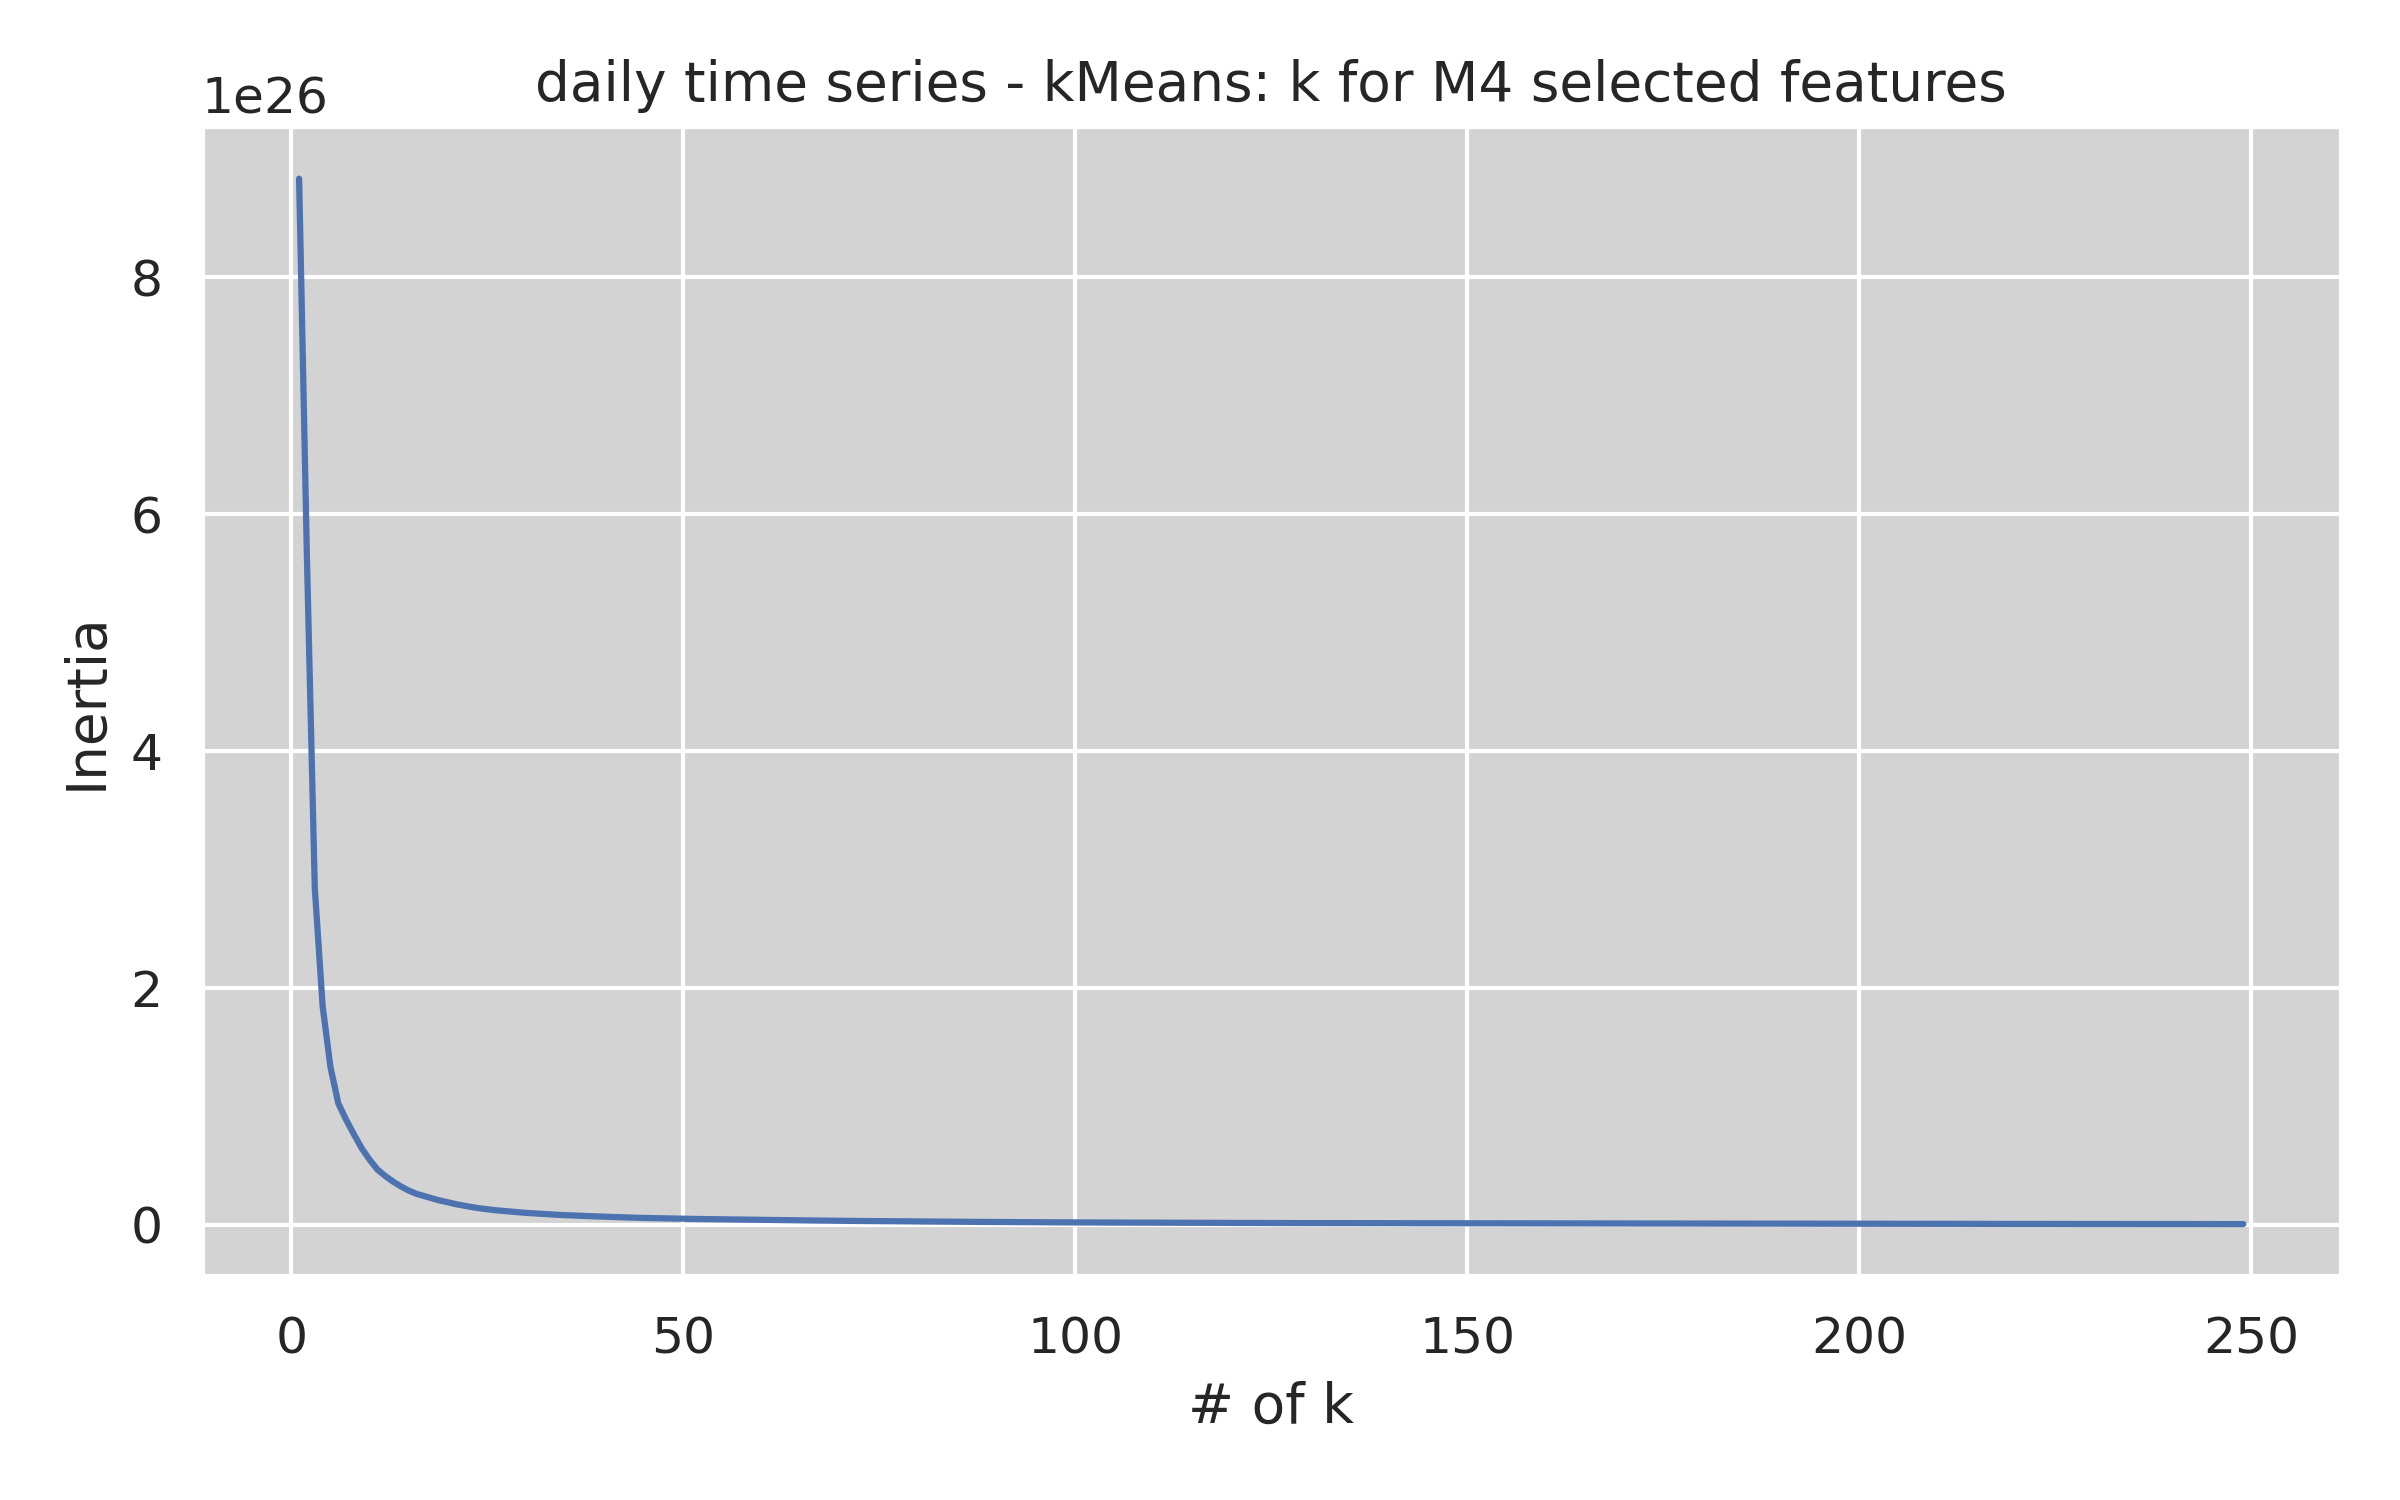
\includegraphics[width=450px]{./img/daily_kmeans_series_inertia.png}
\end{center}
\subsubsection*{Silhouette score}
\label{sec:orge9ba392}
$$ s(i) = \frac{b(i) - a(i)}{{\max\{a(i),b(i)\}}} $$
\begin{center}
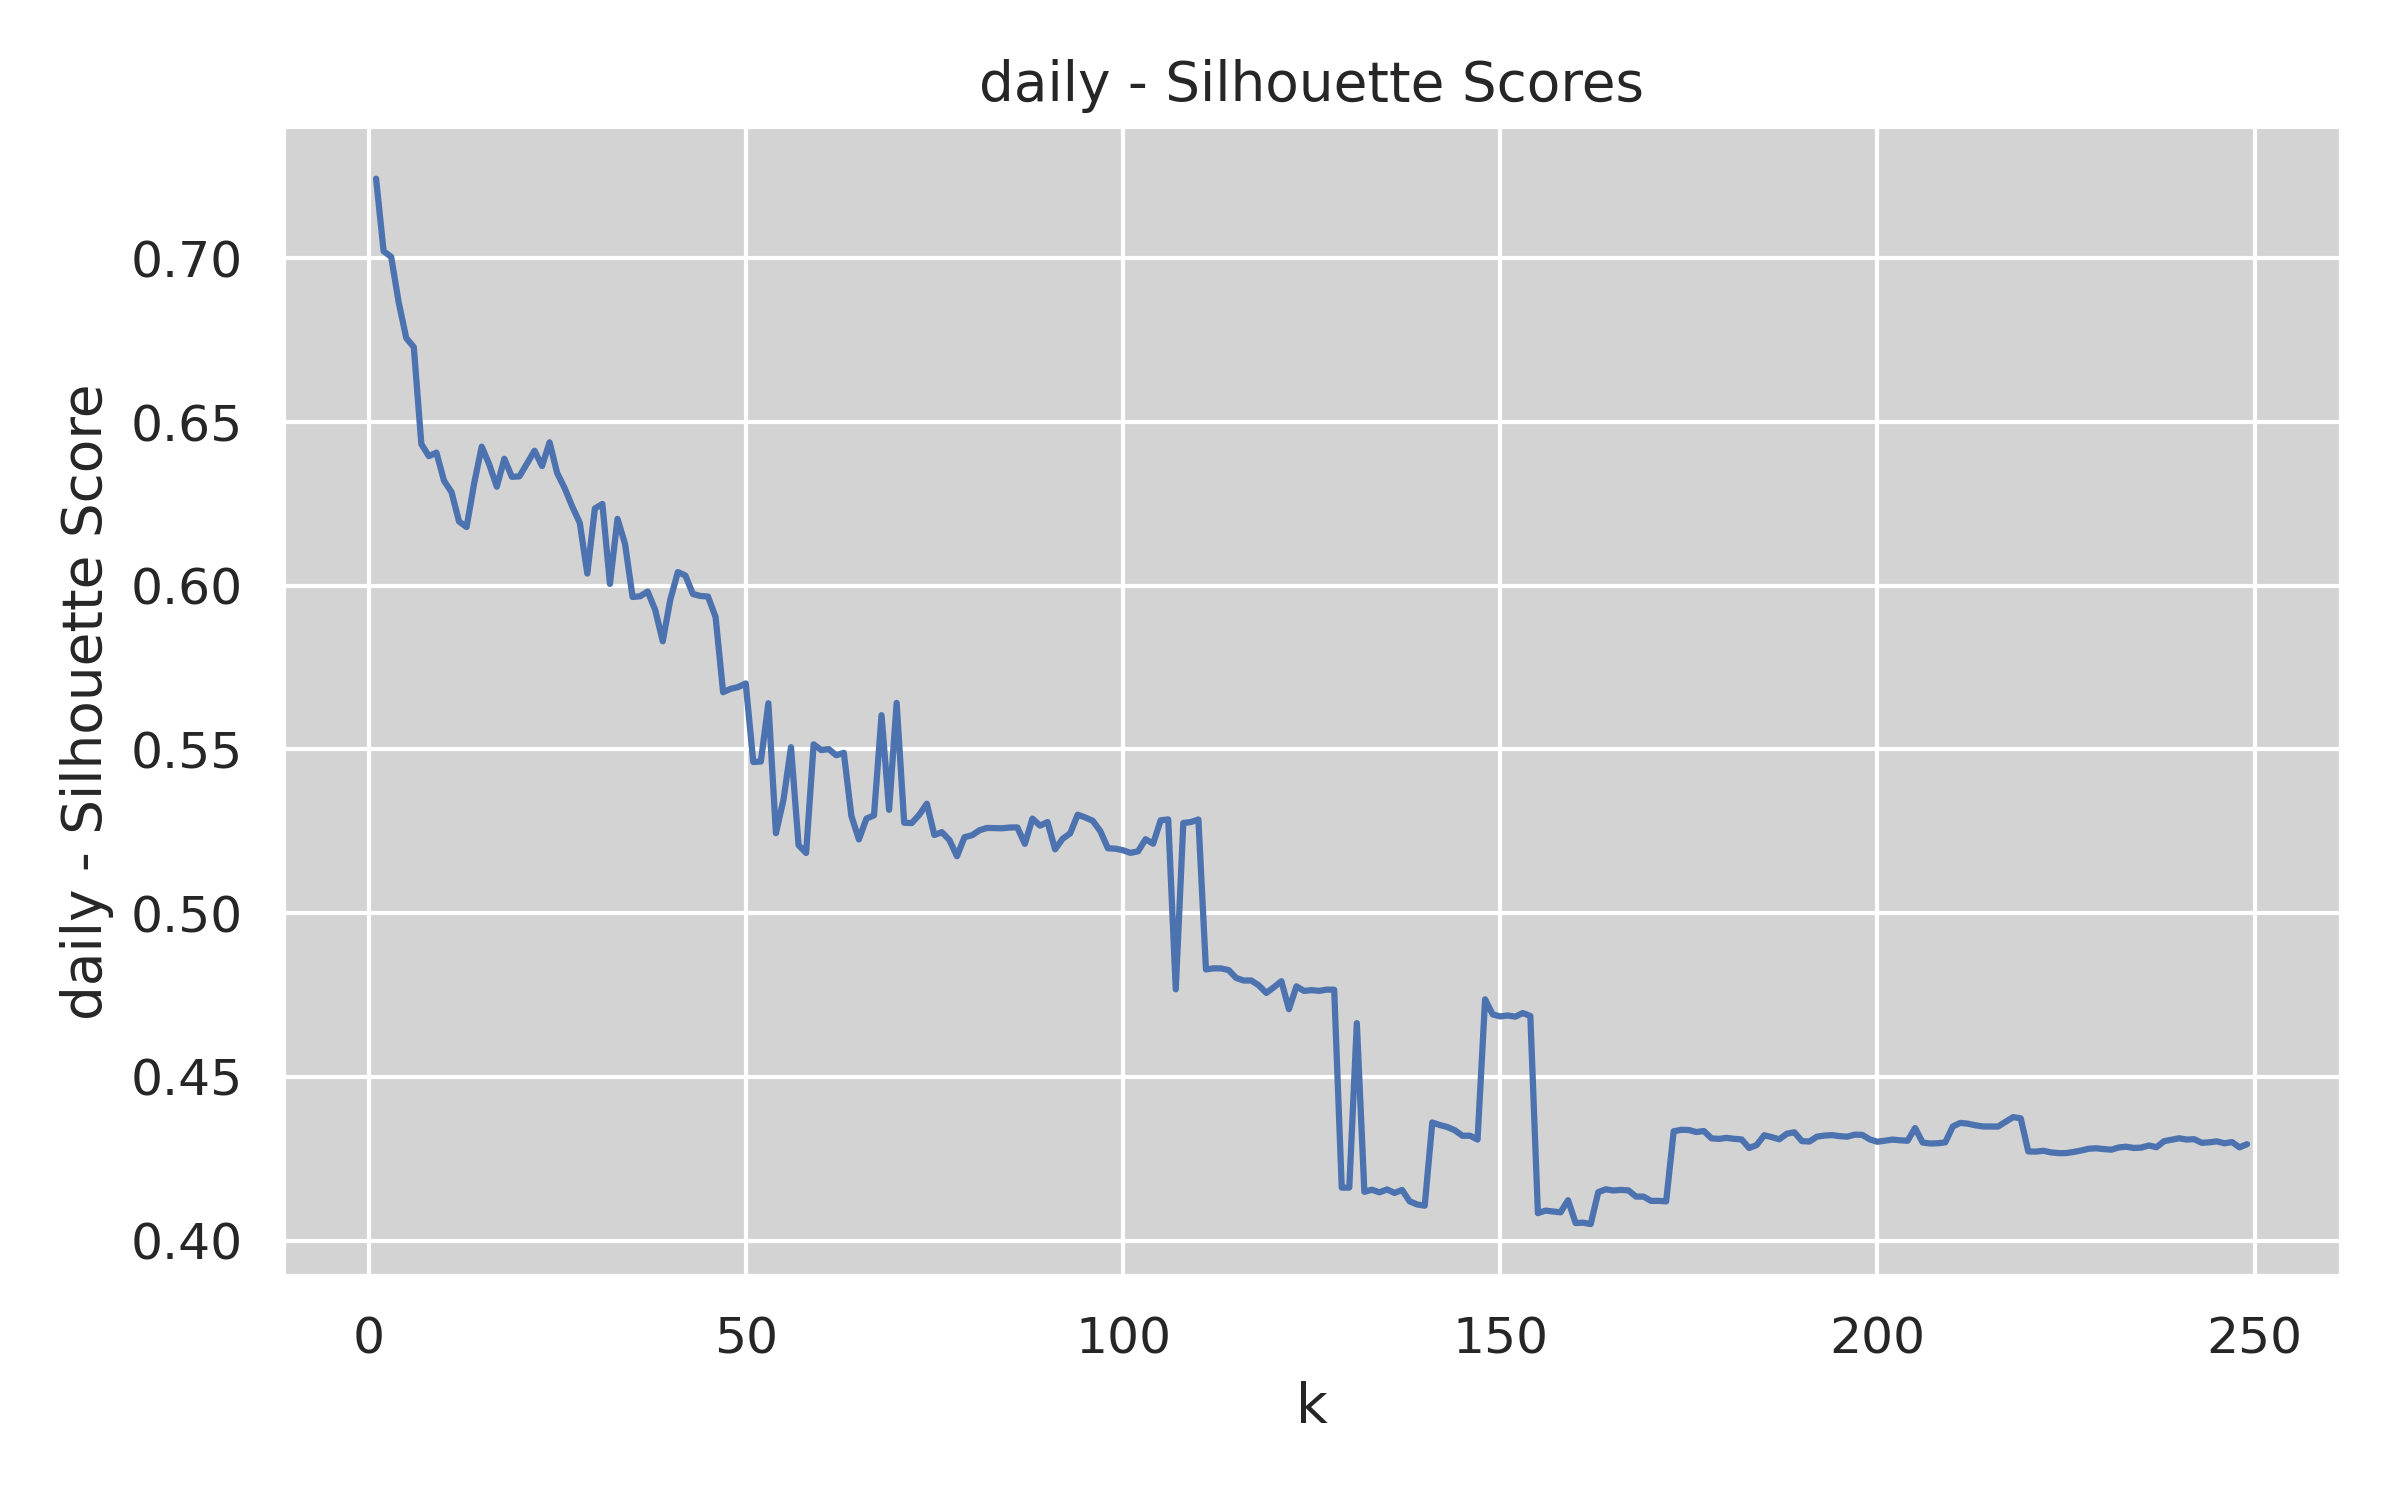
\includegraphics[width=450px]{./img/daily_kmeans_sil_score_series.png}
\end{center}
\subsubsection*{Silhouette Diagrams}
\label{sec:orgea89b3c}
\begin{center}
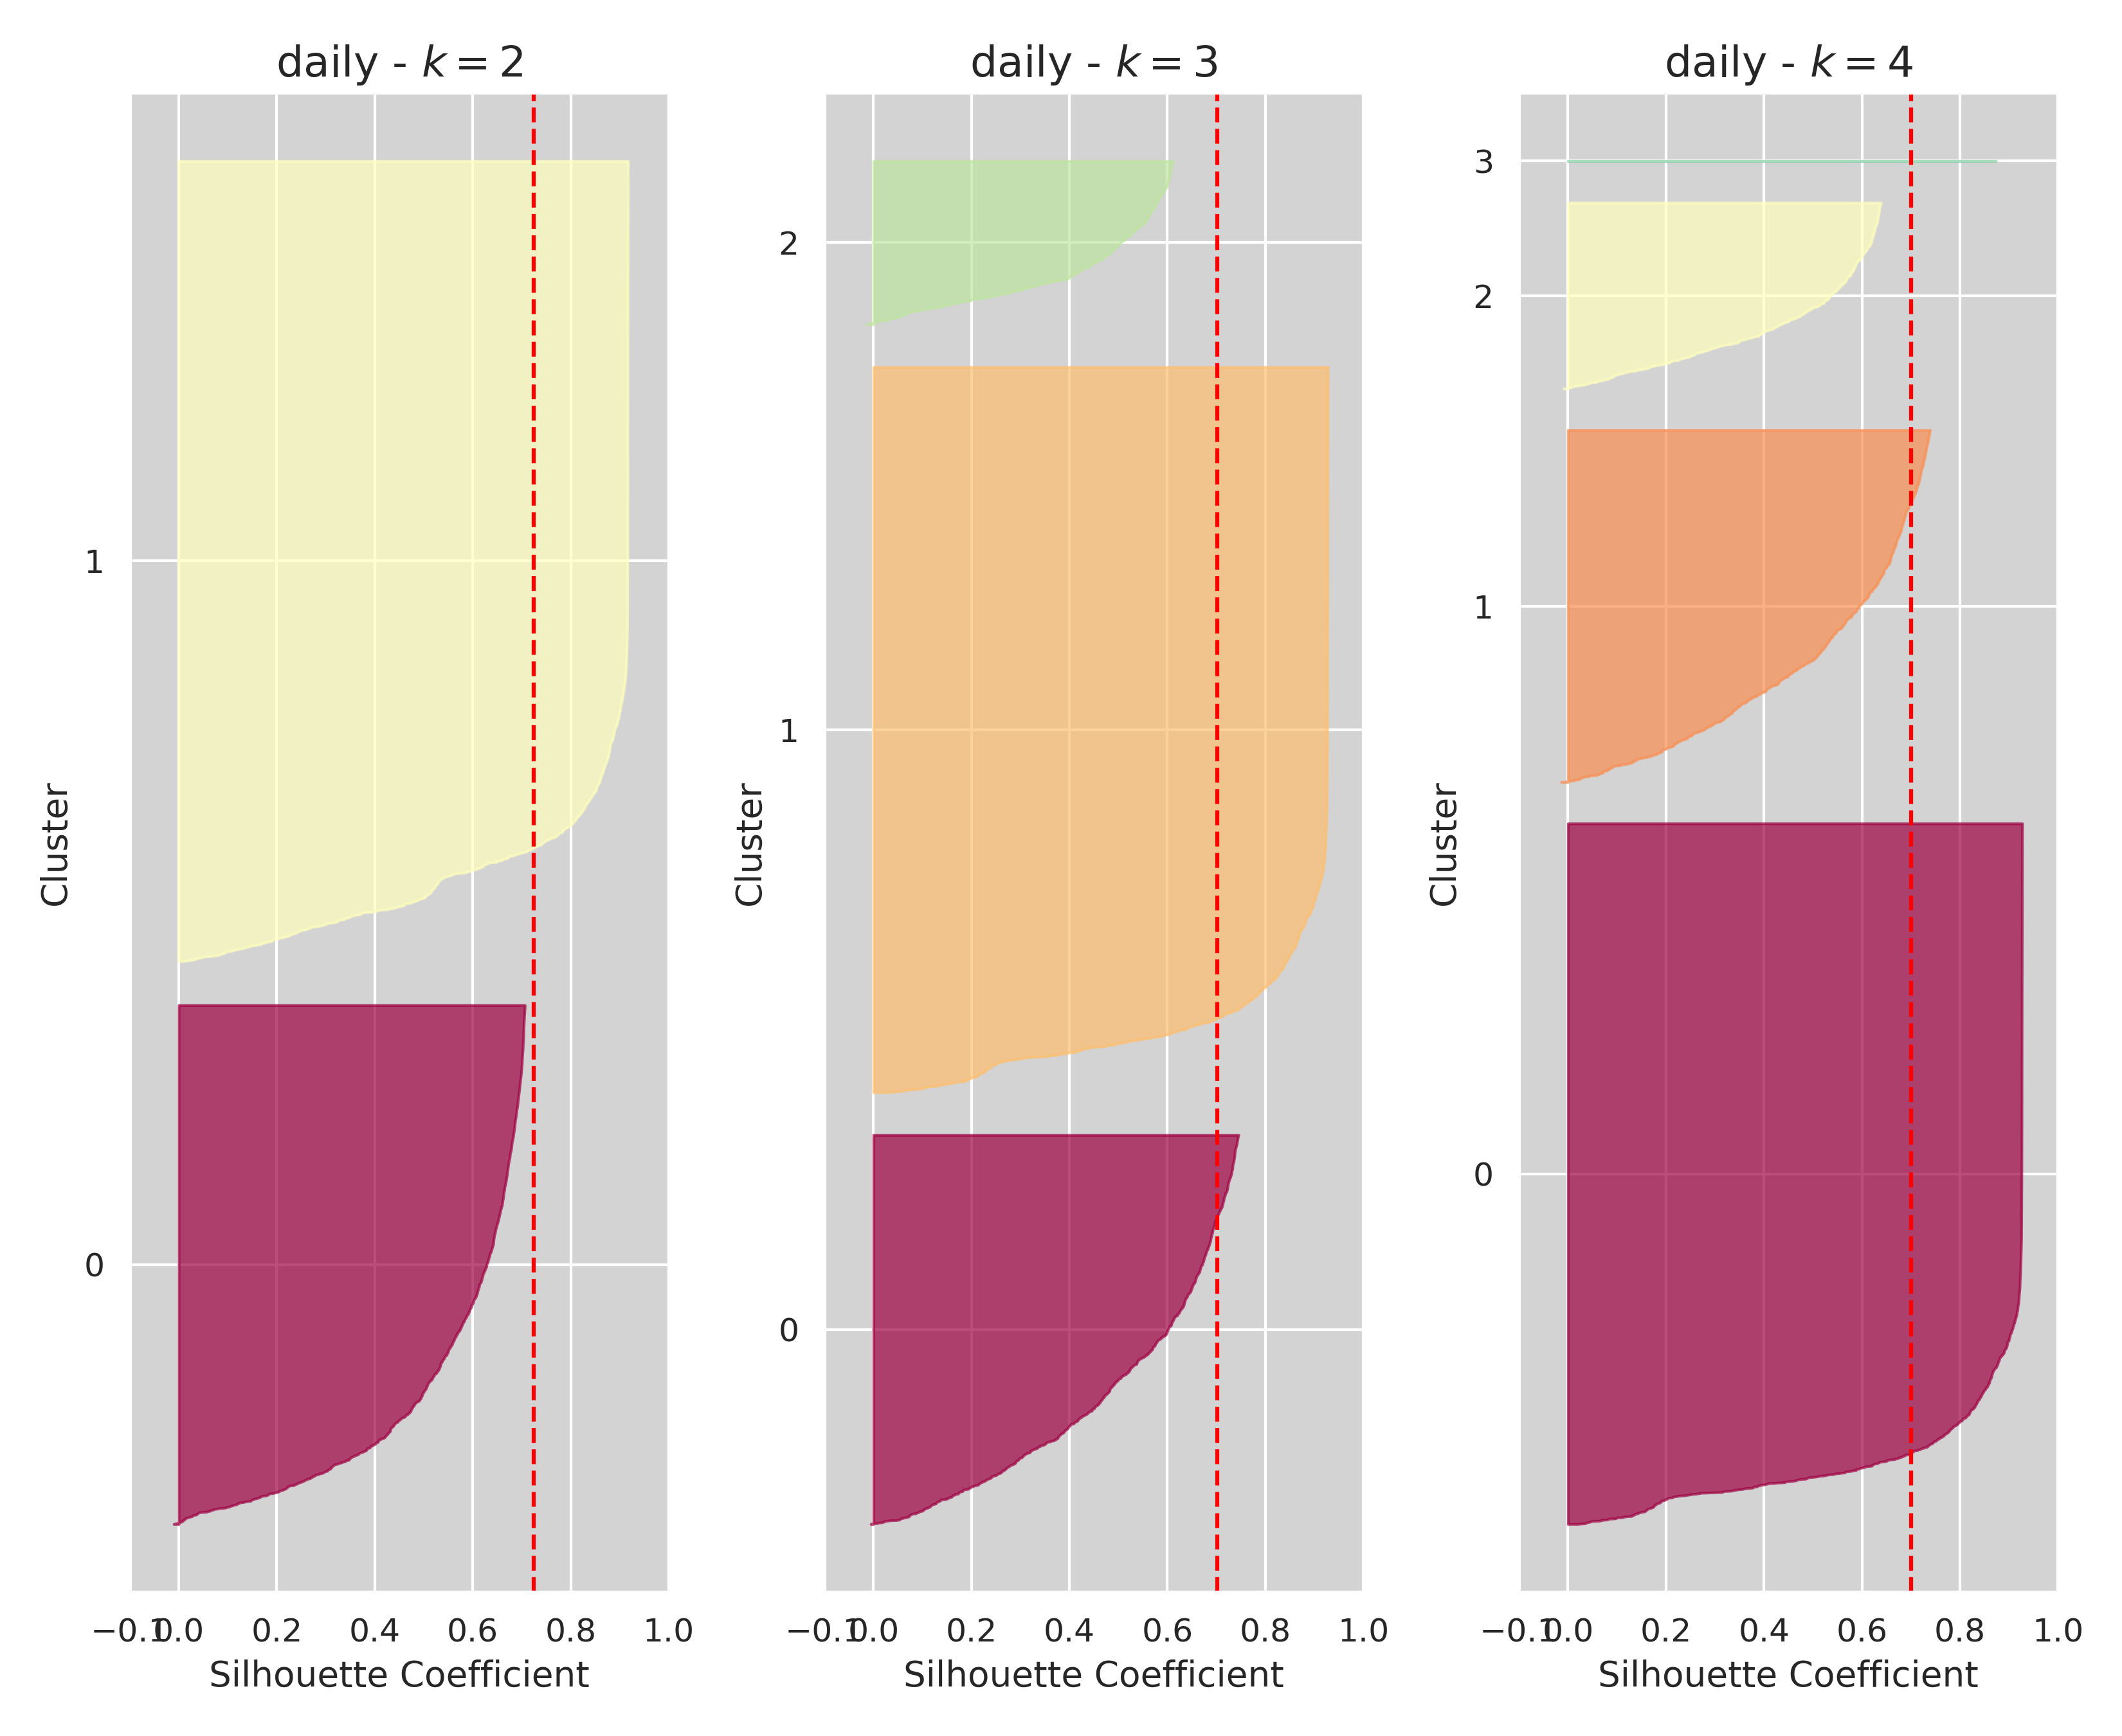
\includegraphics[width=450px]{./img/daily_kmeans_sil_dia_series.png}
\end{center}
\subsection*{Forecasting}
\label{sec:org6e1930c}
\subsubsection*{Neural Network}
\label{sec:org92daa3f}
\begin{itemize}
\item 3 hidden layers
\item features - lags 1 - 7
\item loss: MSE
$$ MSE = \frac{1}{n} \sum_{i=1}^n (Y_i - \hat{Y}_i)^2 $$
\end{itemize}
\subsubsection*{Approach}
\label{sec:org64f874c}
\begin{itemize}
\item full dataset
\item clustered datasets
\item equivalent random datasets
\end{itemize}
\subsubsection*{Cross-Validation}
\label{sec:orgedcb95b}
\begin{itemize}
\item increase certainty about the error that is encountered in the training
\item limit effects of peculiarities in the data on error metrics
\end{itemize}
\subsection*{Benchmarking}
\label{sec:orge7b84ed}
\subsubsection*{M4 Accuracy Metrics}
\label{sec:org3921d7d}
$$ SMAPE = \frac{100}{n} \sum_{t=1}^{n} \frac{F_t - Y_t}{(\lvert F_t \rvert + \lvert Y_t \rvert)/2} $$
$$ MASE = mean \left( \frac{\lvert e_j \rvert}{\frac{1}{T-1} \sum_{t=2}^{T} \lvert Y_t - Y_{t-1} \rvert} \right) $$
\subsection*{Challenges}
\label{sec:org1df2eed}
\subsubsection*{Data Preprocessing}
\label{sec:orga9d24d7}
\begin{itemize}
\item data format - wide vs. long format
\item Min-Max feature scaling with cross validation with neural networks
\item information leakage
\end{itemize}
\subsubsection*{Feature extraction and selection}
\label{sec:org43a3fd8}
\begin{itemize}
\item tsfresh - 800 metrics
\item comprehensive vs. efficient
\end{itemize}
\subsubsection*{Computational Costs}
\label{sec:orgdd853d7}
\begin{itemize}
\item 6 vCPU / 32GB RAM
\item feature extraction and selection (reason for daily only)
\item neural network with cv
\end{itemize}

\subsection*{Results}
\label{sec:orgc1a5651}
\subsubsection*{Cross validation}
\label{sec:orgeaee3a9}
\begin{center}
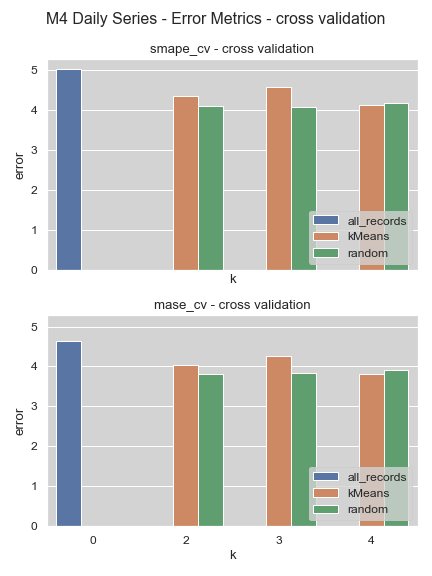
\includegraphics[width=.9\linewidth]{./img/daily_cv_results.png}
\end{center}
\subsubsection*{M4 results}
\label{sec:orgfae6af1}
\begin{center}
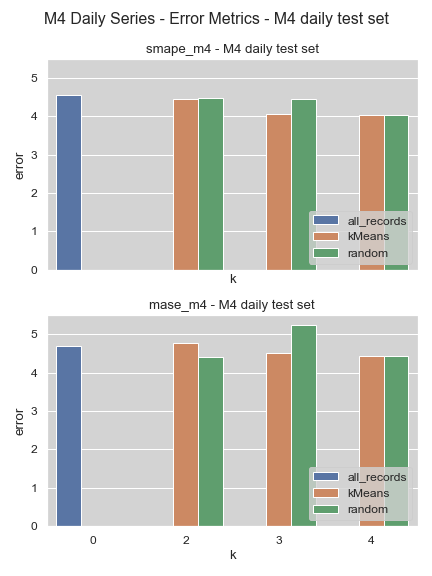
\includegraphics[width=.9\linewidth]{./img/daily_m4_results.png}
\end{center}
\subsection*{Conclusion}
\label{sec:org0b20936}
\begin{itemize}
\item clustering results not better than random
\end{itemize}
\subsubsection*{features vs lags for NN}
\label{sec:org105c8f2}
\begin{itemize}
\item possibly better results
\item increase of neural network size
\item how meaningful are efficient features
\end{itemize}
\subsubsection*{Approach to cross validation}
\label{sec:org2ab1d6d}
\begin{itemize}
\item less folds
\item MinMax scaler
\end{itemize}
\subsubsection*{Uncertainty in the clustering}
\label{sec:org97e2547}
\begin{itemize}
\item reduced uncertainty in the data clustered data
\item indication in MASE (higher in test results compared to cv)
\end{itemize}
\subsubsection*{Complexity of problem definition}
\label{sec:org5d9740c}
\begin{itemize}
\item many moving parts
\item \href{https://github.com/philippbeer/m4\_clustering}{M4 Clustering on Github}
\end{itemize}
\subsection*{Outlook}
\label{sec:orgd1d702f}
\begin{itemize}
\item Algorithm
\label{sec:org9231f1f}
\begin{itemize}
\item hierarchical and density and grid-based methods
\end{itemize}
\item Feature Choice
\label{sec:orgbe56351}
\begin{itemize}
\item ranking of features
\end{itemize}
\end{itemize}
\subsection*{Thank you for your attention}
\label{sec:orgba35993}
\end{document}